\newcommand{\stepbox}[2]{\alt<#1>{\boxed{#2}}{#2}}

\begin{frame}
	{Preliminary Phase: Approximating \(\mathcal{D}_\text{train}\)'s decision boundary}
	\small

	\begin{figure}
		\centering
		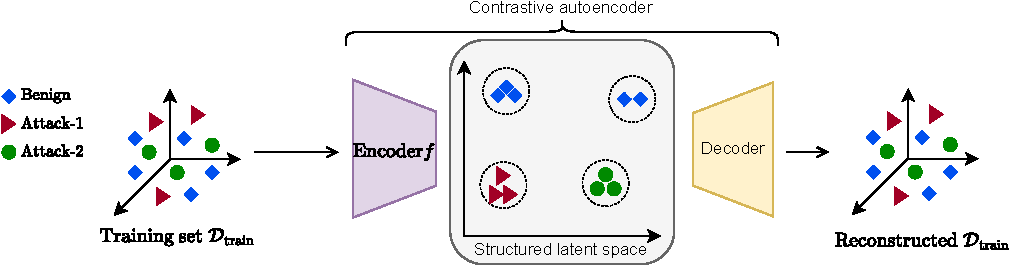
\includegraphics[width=\linewidth]{sections/TATA/methodology/figures/TATA_pre-crop}
		%    \caption*{
		%      \scriptsize{Encoder \(f\) and its associated decoder trained on
		%        \(\mathcal{D}_{\text{train}}\) to construct a structured latent
		%        space \(\mathcal{Z}_{\text{train}}=\{\,z \mid z=f(x;\theta),\ x\in
		%        \mathcal{D}_{\text{train}}\}\).}
		%    }
		\label{fig:tata_preliminary}
	\end{figure}

	\begin{itemize}
		%    \item Latent space under contrastive autoencoder: well-separated clusters
		%    \(C_{i,\,l_k} \in \mathcal{C}\); majority label \(l_k\) per cluster.
		%
		%    \item Dimensionality reduction; accelerated later phases; model-agnostic
		%    approximation of \(\mathcal{D}_{\text{train}}\) decision boundaries.

		\item Decision boundaries \(\approx\) cluster borders in the latent space; these
		      are captured in the encoder’s weights.

	\end{itemize}

\end{frame}

%\begin{frame}{Preliminary Phase: Approximating \(\mathcal{D}_\text{train}\)
%  's decision boundary}
%  \small
%  \begin{minipage}[t]{0.38\textwidth}
%    \begin{itemize}
%
%      \item Latent space under contrastive autoencoder: well-separated clusters
%      \(C_{i,\,l_k} \in \mathcal{C}\); majority label \(l_k\) per cluster.
%
%      \item Dimensionality reduction; accelerated later phases; model-agnostic
%      approximation of \(\mathcal{D}_{\text{train}}\) decision boundaries.
%
%    \end{itemize}
%  \end{minipage}
%  \hfill
%  \begin{minipage}[t]{0.6\textwidth}
%    \begin{figure}
%      \centering
%      
\includegraphics[width=1.1\linewidth]{tata/figures/TATA_pre-crop}
%      \caption*{
%        \scriptsize{Encoder \(f\) and its associated decoder trained on
%          \(\mathcal{D}_{\text{train}}\) to construct a structured latent
%          space \(\mathcal{Z}_{\text{train}}=\{\,z \mid z=f(x;\theta),\ x\in
%          \mathcal{D}_{\text{train}}\}\).}}
%      \label{fig:tata_preliminary}
%    \end{figure}
%  \end{minipage}
%\end{frame}

\begin{frame}{Phase 1: Test-set Assessment}
	\small
	\begin{minipage}[t]{0.48\textwidth}
		\begin{itemize}

			\item Encode $\mathcal{D}_{\text{train}}$ \& $\mathcal{D}_{\text{test}}$
			      $\rightarrow$ $\mathcal{Z}_{\text{test}}$ is located relative to
			      $\mathcal{Z}_{\text{train}}$ $\rightarrow$ we now work entirely in latent space
			      (\(\mathcal{Z}_{\text{train}},\mathcal{Z}_{\text{test}}\)).



			\item[]

			\item For each test embedding \(z\), we identify:
			      \begin{itemize}
				      \item \(P(z)\): the nearest \textbf{same-label cluster} (\emph{positive
					            cluster})
				      \item \(N(z)\): the nearest \textbf{different-label cluster} (\emph{negative
					            cluster})
			      \end{itemize}

			\item[]


			\item Define proximity, diversity, and scarcity per \(P(z)\)
			      ; then aggreate.

		\end{itemize}
	\end{minipage}
	\hfill
	\begin{minipage}[t]{0.48\textwidth}
		\begin{figure}
			\centering
			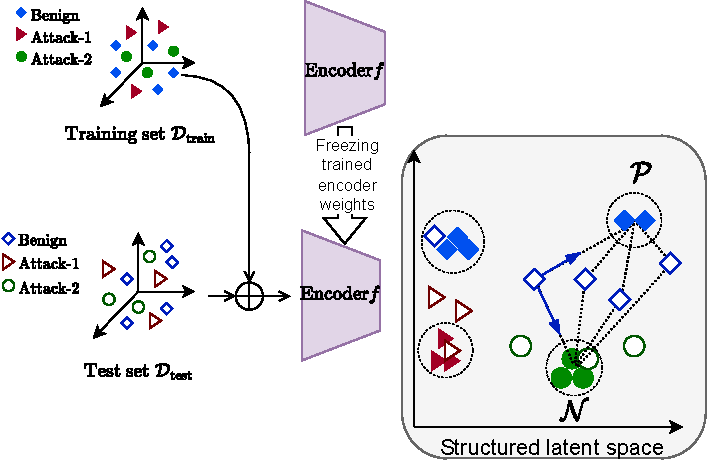
\includegraphics[width=\linewidth]
			{sections/TATA/methodology/figures/TATA_phase_1-crop}
			%      \caption*{\scriptsize{Assesing \(\mathcal{D}_{\text{test}}\) quality}}
			\label{fig:tata_phase_1}
		\end{figure}
	\end{minipage}
\end{frame}

\input{sections/TATA/methodology/metrics}


% --- Preamble (if not already added) ---
\newcommand{\strike}[1]{\textcolor{red!70!black}{\sout{#1}}}

% --- Frame ---
\begin{frame}{Which approaches can augment the test set?}
	\small

	\begin{enumerate}
		% 1) Synthetic generation (as before; crossed on next click)
		\item<1->
		      \alt<2->{\strike{GANs / diffusion models.}}
		      {GANs / diffusion models.}
		      \begin{itemize}
			      \item<2-> Synthetic generation may break protocol semantics $\Rightarrow$
			            unrealistic flows.
		      \end{itemize}

		      \vspace{0.6em}

		      % 2) Network simulators
		\item<3-> \alt<4->{\strike{Network simulators (e.g., NS-3, OMNeT++)}}
		      {Network simulators (e.g., NS-3, OMNeT++)}
		      \begin{itemize}
			      \item<4->
			            Models protocol interactions, offering more realism.
			      \item<4-> Remaining realism gap vs.\ real hardware and user behavior.
		      \end{itemize}

		      \vspace{0.6em}

		      % 3) Live testbed
		\item<5-> Using a \textbf{configurable live testbed}.
		      \begin{itemize}
			      \item<6-> Best preserves realism of generated traffic.
			      \item<6->
			            Emits legitimate traffic across multiple protocols (HTTP/HTTPS, SSH, SMTP, DNS,
			            \dots) and can generate attack traffic under controlled conditions.
		      \end{itemize}

		      \vspace{0.6em}

		      % This uncover block makes the colored box appear on the 9th click
		      \uncover<7->{
			      \setbeamercolor{focusbox}{use={structure, normal text},
			      fg=structure.fg,
			      bg=structure.fg!12!normal text.bg}
		      \begin{beamercolorbox}[wd=\linewidth, sep=1ex, rounded=true]{focusbox}
			      \small
			      Generate targeted configs so the testbed produces realistic flows targeting
			      under-covered \(\mathcal{Z}\) regions (low \(D,P,S\)).
		      \end{beamercolorbox}
		      }
	\end{enumerate}

\end{frame}

%\begin{frame}{Phase 2: Targeted Augmentation}
%  \scriptsize
%  \begin{minipage}[t]{0.52\textwidth}
%    \begin{itemize}
%
%      \item Start from Preliminary \& Phase 1 outputs
%      \item[]
%
%      \item \textbf{Train the agent (DRL):}
%
%      \begin{itemize}
%        \scriptsize
%        \item \textbf{Observation} \(o_t\): centroids \(\mathcal{C}\)
%        + basic stats of current \(\mathcal{Z}_{\text{test}}\)
%        (mean/min/max/var/std).
%        \item \textbf{Action} \(a_t\)
%        : select a testbed configuration (e.g., delay / loss / duplication).
%        \item \textbf{Reward} \(r_t\): \(D,P,S\).
%
%        \item \textbf{Training workflow}:
%        \[
%          \begin{aligned}
%            \stepbox{1}{o_t} &\;\to\; \stepbox{2}{a_t} \;\to\; \stepbox{3}{x_t}
%            \;\xrightarrow{\,f\,}\; \stepbox{4}{z_t} \;\to\;
%            \stepbox{5}{\text{update }\mathcal{Z}_{\text{test}}} \\
%            &\;\to\; \stepbox{6}{(r_t,\,o_{t+1})} \;\to\;
%            \stepbox{7}{\text{update }\pi}\;\stepbox{8}{\circlearrowright}
%            \;\Rightarrow\; \stepbox{9}{\pi^\ast}
%          \end{aligned}
%        \]
%
%      \end{itemize}
%
%      \item Apply \(\pi^\ast\) to augment any
%      \(\mathcal{D}_{\text{test}}\)
%    \end{itemize}
%  \end{minipage}
%  \hfill
%  \begin{minipage}[t]{0.47\textwidth}
%    \begin{figure}
%      \centering
%      
\includegraphics[width=1.1\linewidth]{tata/figures/TATA_phase_2_light-crop}
%%      \caption*{\scriptsize{Phase 2: targeted augmentation of
%%        \(\mathcal{D}_{\text{test}}\)
%%        using Preliminary + Phase 1 results.}}
%      \label{fig:tata_phase_2}
%    \end{figure}
%  \end{minipage}
%\end{frame}


\begin{frame}[t]{Phase 2: Targeted Augmentation}
	\scriptsize

	% --- top figure ---
	\begin{center}
		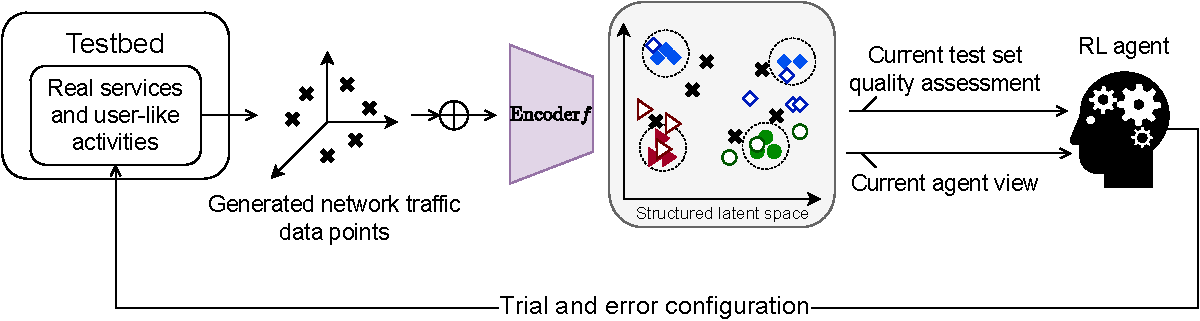
\includegraphics[width=0.95\linewidth]{sections/TATA/methodology/figures/TATA_phase_2_light-crop}
	\end{center}
	\vspace{0.4em}

	% --- text below ---
	\begin{itemize}
		\item Start from Preliminary \& Phase 1 outputs
		\item []
		\item \textbf{Training workflow}:
		      \[
			      \begin{aligned}
				      \stepbox{1}{\text{observe latent-space}} & \;\to\;
				      \stepbox{2}{\text{select a configuration}} \;\to\;
				      \stepbox{3}{\text{traffic generation}}
				      \;\xrightarrow{\;\text{embed}\;}\;
				      %        \stepbox{4}{\text{get latent embedding}} \;\to\; \\
				      \stepbox{4}{\text{update } \mathcal{Z}_{\text{test}}}                                                             \\
				                                               & \;\to\; \stepbox{5}{\text{compute proximity, diversity, and scarcity}}
				      \;\to\; \stepbox{6}{\text{update policy } \pi} \;\stepbox{7}{\circlearrowright}
				      \;\Rightarrow\; \stepbox{8}{\pi^\ast}
			      \end{aligned}
		      \]
		      %    \item []
		      %    \[
		      %      \begin{aligned}
		      %        \stepbox{1}{o_t} &\to \stepbox{2}{a_t} \to \stepbox{3}{x_t}
		      %        \xrightarrow{\,f\,} \stepbox{4}{z_t} \to
		      %        \stepbox{5}{\text{update }\mathcal{Z}_{\text{test}}}
		      %        &\to \stepbox{6}{(r_t,\,o_{t+1})} \to
		      %        \stepbox{7}{\text{update }\pi}\;\stepbox{8}{\circlearrowright}
		      %        \Rightarrow \stepbox{9}{\pi^\ast}
		      %      \end{aligned}
		      %    \]
		\item Apply \(\pi^\ast\) to augment any \(\mathcal{D}_{\text{test}}\)
	\end{itemize}
\end{frame}


%\begin{frame}{TATA}
%  \begin{figure}
%    \centering
%    \includegraphics[width=0.7\linewidth]
%    {tata/figures/TATA-crop}
%    \caption{Example Figure}\label{fig:tata_overview}
%  \end{figure}
%\end{frame}
